\documentclass[12pt]{article}
\usepackage{geometry}
\usepackage{graphicx}
\usepackage{amsmath}
\usepackage{fancyhdr}
\usepackage{hyperref}
\usepackage{booktabs}    % For professional-looking tables
\usepackage{array}       % For extended column definitions
\usepackage{tabularx}    % For adjustable-width tables
\usepackage{longtable}


\geometry{margin=1in}

\title{Aircraft Design 1 - Fall 2024 \\ Assignment 1}
\author{Smythe Cy Goforth Jr, Matthew Burnett \\ Group 6 \\ Instance: [first delivery]}
\date{Hours spent on assignment: [35]}

\begin{document}
	
	\maketitle
	
	\section*{Aircraft Type: UAV}
	\textbf{Aircraft Number: Glider UAV Project}
	
	\begin{table}[h!]
		\centering
		\begin{tabular}{|l|c|c|}
			\hline
			Reference Type & Value & Unit \\ 
			\hline
			Payload & 11.02 & lb \\ 
			Range & 6.21 & mi \\ 
			Altitude & 400 & ft \\ 
			Cruise Speed & 49.21 & ft/s \\ 
			Ceiling & 4000 & ft \\ 
			Endurance & 3 & Hours \\ 
			Max Speed & 65.62 & ft/s \\ 
			Max Weight & 55.02 & lb \\ 
			\hline
		\end{tabular}
		\caption{Basic Aircraft Specifications}
	\end{table}
	
	\newpage
	
	\tableofcontents
	
	\newpage
	
	
	\section{Mission Definition and Analysis of Requirements}
	The Low Altitude High Endurance Unmanned Aerial Vehicle (LAHE UAV) is intended to serve as a robust and versatile platform for scientific observation and environmental monitoring. To perform this role, the LAHE UAV must be optimized for three primary factors.
	
	\begin{enumerate}
		\item \textbf{Endurance:} For environmental monitoring and scientific observation, it is crucial that the aircraft can stay airborne long enough to perform tests. 
		\item \textbf{Payload Weight:} To host a wide variety of sensor equipment, it is important to provide sensor package development teams with an ample weight budget.
		\item \textbf{Payload Volume:} The UAV must also be able to host packages of varying volume.
	\end{enumerate}
	
	This chapter will explore FAA requirements for low-altitude UAV systems, payload specifications, and necessary design considerations.
	
	\subsection{The Mission}
	The mission for the LAHE UAV is centered around observation. The aircraft will be launched by a single operator in a remote environment, climbing to a cruise altitude of 1312.34 ft and maintaining a cruise speed of 32.81 ft/s. Once the cruise altitude is reached, the aircraft will enter the observation phase, where the payload will be utilized. The mission continues until the observation is complete, followed by a return to the operator, and a controlled descent and landing.
	
	\begin{figure}[h!]
		\centering
		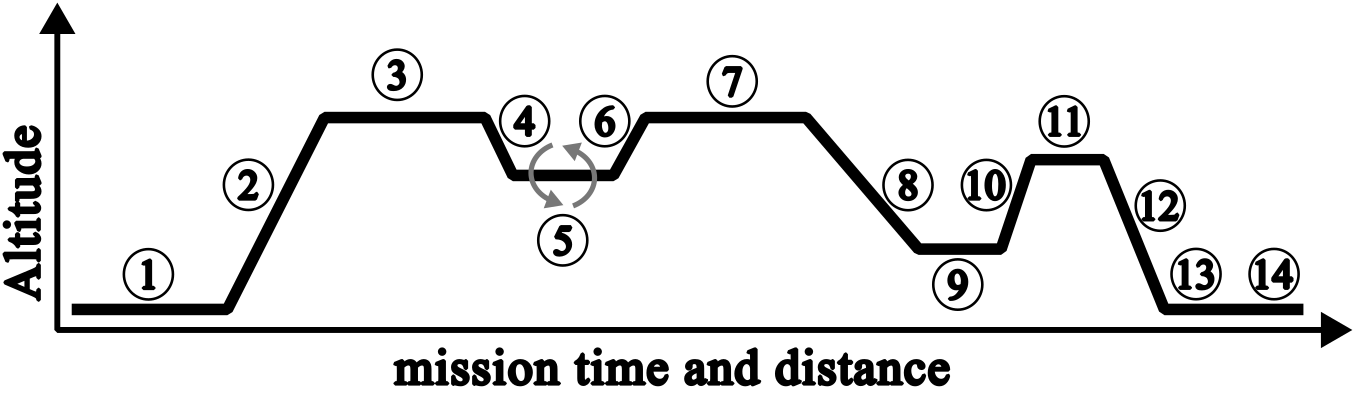
\includegraphics[width=4.5 in]{Media/MissonPlan.png} % Placeholder for technical drawings
		\caption{Technical drawings: top, side, and front views of the fuselage}
	\end{figure}
	
	\begin{enumerate}
		\item \textbf{Start Motor/s and Takeoff}: The LAHE UAV will be launched via a catapult system using an internal lithium-ion battery to power its electric motor, allowing for rapid deployment in remote environments.
		
		\item \textbf{Climb to Cruise Altitude}: The UAV will climb to 400 ft at a low angle of attack to avoid stalling due to the glider airfoil design.
		
		\item \textbf{Cruise to Survey Area}: Upon reaching cruise speed and altitude, the UAV will travel to the survey area.
		
		\item \textbf{Descend to Survey Area}: The UAV will begin its descent to the survey area while carefully managing its angle of attack to prevent stalling.
		
		\item \textbf{Loiter at Survey Area}: Once at the desired altitude, the UAV will alternate between powered flight and gliding while loitering.
		
		\item \textbf{Ascend Back to Cruise Altitude}: After completing the loiter phase, the UAV will ascend back to its cruise altitude for the return trip.
		
		\item \textbf{Cruise Back to Landing Zone}: The UAV will travel back to the designated landing area, maintaining its cruise speed and altitude.
		
		\item \textbf{Descend to Landing Zone}: The UAV will descend steadily with a minimal angle of attack to prepare for landing.
		
		\item \textbf{Attempt Landing}: The UAV will attempt a soft landing by reducing its power and using a gliding approach.
		
		\item \textbf{Abort Landing if Necessary}: If conditions are not suitable, the UAV will abort its landing attempt and return to loiter over the landing zone.
		
		\item \textbf{Loiter Over Landing Zone}: The UAV will loiter and circle over the landing area, waiting for optimal landing conditions.
		
		\item \textbf{Final Descent for Landing}: After loitering, the UAV will perform a final descent with precision control.
		
		\item \textbf{Landing}: The UAV will land with fixed gear.
		
		\item \textbf{Power Off and Recover Equipment}: After landing, the UAV will power down, and the sensor equipment is recovered.
	\end{enumerate}
	
	\subsection{Requirement Analysis}
	\subsubsection{Payload Analysis}
	The UAV's payload consists of a wide variety of sensor equipment. Ports will be placed in the removable top section of the fuselage to make exterior readings. With approximately 3 cu ft
	
	\begin{table}[h]
		\centering
		\caption{Aircraft Specifications}
		\begin{tabular}{|l|l|l|}
			\hline
			\textbf{Aircraft} & \textbf{Battery Capacity} & \textbf{Payload} \\ 
			\hline
			SITARIA E & 73.5 Ah & 8.82 lb \\ 
			\hline
			\textbf{LAHE UAV} & \textbf{80 Ah} & \textbf{11.02 lb} \\ 
			\hline
			BOREY 20 & 83 Ah & 11.02 lb \\ 
			\hline
		\end{tabular}
	\end{table}
	
	\subsubsection{Propulsion Analysis}
	With a proposed cruise speed of 32.81 ft/s and a payload of 11.02 lb, the propulsion will be provided by a brush-less electric motor. A balance between motor weight and torque output is necessary. Future work will optimize the motor and propeller selection.
	
	\subsubsection{Certification Analysis}
	To accommodate end users who don't possess commercial UAV licenses, the drone must be able to fly within unregulated airspace and be under regulated weights. According to FAA regulations, to fly a UAV unlicensed, the UAV must weigh under 55.12 lb, fly within visual line of sight (within 3 miles), and under 400 ft of altitude. The UAV will be designed to operate above this ceiling and beyond that range to also meet the needs of licensed end users.
	
	\subsubsection{Range, Takeoff, and Landing Distance}
	The UAV must cover a range of 6.21 mi. Its endurance will be extended through efficient gliding, with minimal battery power used for propulsion.
	
	\subsubsection{Additional Requirements}
	Other requirements include minimizing power consumption, maximizing endurance, and maintaining FAA certification.
	
	\subsection{Driving Requirements}
	The critical requirements for the UAV design include range, endurance, and payload capacity, all of which influence the motor choice.
	
	\section{Reference Aircraft Data Collection}
	A range of reference aircraft were studied for inspiration and comparison. Few aircraft are designed for the same mission as the LAHE UAV. Aircraft were selected for meeting a few or all of the same criteria. Some, for example, have the same approximate payload and operational ceiling but pose gas engines making their range woefully longer. These aircraft are nonetheless useful to study so long as the differences are acknowledged. The full reference list is included in Appendix A. Below are a selected few reference aircraft that match the LAHE UAV mission well.
	\newpage
	\begin{table}[h!]
		\centering
		\caption{Reference Aircraft Data}	
		\label{tab:reference_aircraft_data}
		\begin{tabular}{@{} 
				>{\raggedright\arraybackslash}p{3cm} 
				>{\raggedright\arraybackslash}p{3cm} 
				>{\centering\arraybackslash}p{2cm} 
				>{\raggedright\arraybackslash}p{3cm} 
				>{\centering\arraybackslash}p{2cm} 
				>{\raggedright\arraybackslash}p{3cm} 
				@{}}
			\toprule
			\textbf{Aircraft Name} & \textbf{Payload} & \textbf{Range} & \textbf{Cruise Speed} & \textbf{Type of Power Plant} & \textbf{Endurance} \\ 
			\midrule
			Albatross Fixed Wing UAV & 9.7 lb & 62.14 mi & 42.33 mph & Lithium Ion Electric & 4 hr \\ 
			\midrule
			SAT-i & 1.32 lb & 155.34 mi & 17.78 ft/s & Electric 400W & 2 hours \\ 
			\midrule
			SITARIA E & 
			\begin{tabular}[c]{@{}l@{}}Nominal Payload:\\ 8.82 lb\\ Max payload:\\ 22.05 lb\end{tabular} 
			& 149.13 mi & 49.71 mph & 
			\begin{tabular}[c]{@{}l@{}}Electric\\ 2.5 kW\\ Battery:\\ 73.5 Ah\end{tabular} 
			& 
			\begin{tabular}[c]{@{}l@{}}8.82 lb Payload\\ 3 h\\ 22.05 lb Payload\\ 1.5 h\end{tabular} \\ 
			\midrule
			BOREY 20 & 8.82 lb & 248.55 mi & 65.62 ft/s & 24V, LI-Ion Electric motor 2000W & 5 hours \\ 
			\bottomrule
		\end{tabular}
	\end{table}
	
	\section{Concept Generation and Selection}
	\subsection{Concept Generation}
	Three design concepts were considered:
	
	\begin{itemize}
		\item Mono-pusher with inverted V-tail
		\item Dual pusher with V-tail
		\item Dual puller with cross-tail
	\end{itemize}
	
	Each concept was designed with a similar internal fuselage layout, while varying in motor and tail configurations. 'Inside-Out' sizing of the fuselage was performed after the concept selection stage.
	
	\newpage
	
	\subsubsection{Mono-pusher with Inverted V-tail}
	\begin{figure}[h!]
		\centering
		\includegraphics[width=6.5 in]{Media/MonoPusherFig.png} % Placeholder for technical drawings
		\caption{(a) The Bayraktar TB2 UAV, designed for medium altitude-long endurance surveillance and payload deployment missions \cite{}. (b) A preliminary design of a mono pusher inverted V-tail configuration.}
	\end{figure}
	Inspired by the Bayraktar TB2, this design features a single rear-facing motor and inverted V-tail.
	
	\textbf{Pros:}
	\begin{itemize}
		\item \textbf{Higher endurance}: Preliminary calculations suggest one engine is sufficient \ref{}. Eliminating the redundant hardware of a second engine saves on weight and, by extension, increases fuel economy. The endurance is further aided by the reduction in drag experienced by V-tail systems. By eliminating one of the three control surfaces on a conventional configuration, the drag is inevitably reduced. 
		\item \textbf{Improved structural rigidity}: The twin boom configuration considerably increases the torsional and bending rigidity of the tail section.
	\end{itemize}
	
	\textbf{Cons:}
	\begin{itemize}
		\item \textbf{Less control authority}: The reduction in control surface area reduces control authority. They are also very prone to adverse roll \cite{}.
		\item \textbf{Inefficient Yaw and Pitch}: The angled nature reduces the authority in these axes \cite{}.
	\end{itemize}
	
	To summarize, this design offers promising structural and flight efficiency characteristics but suffers in its flight control characteristics.
	
	\newpage
	
	\subsubsection{Twin Pusher with V-tail}
	\begin{figure}[h!]
		\centering
		\includegraphics[width=6.5 in]{Media/TwinPusherFig.png} % Placeholder for technical drawings
		\caption{(a) The P.180, designed for medium altitude business travel. (b) A preliminary design of a mono-pusher inverted V-tail configuration.}
	\end{figure}
	Inspired by the Piaggio P.180 Avanti, this concept uses twin rear-facing motors and a V-tail. It should be noted that the P.180 does not possess a V-tail. V-tail configurations in commercial aviation are rare. Extensive literature review yielded no aircraft with a V-tail and a twin pusher. 
	
	\textbf{Pros:}
	\begin{itemize}
		\item \textbf{Increased thrust}: Added thrust would enable heavier payloads and significantly reduce take-off lengths required.
		\item \textbf{Redundancy}: Having two motors would decrease the likelihood of total engine loss.
	\end{itemize}
	
	\textbf{Cons:}
	\begin{itemize}
		\item \textbf{Reduced endurance}: The increased weight and power draw of running two motors would likely reduce the maximum endurance of the UAV.
		\item \textbf{Turbulence on control surfaces}: The pusher configuration would blow high velocity, turbulent air directly on the control surfaces. This turbulent flow could lead to reduced control authority depending on the exact aerodynamics of the aircraft.
	\end{itemize}
	
	To summarize, this design offers the potential of heavier payloads and reduced take-off runs. It also boasts more redundancy than the mono-prop design. This design, however, would likely have decreased maximum endurance and flight performance. The poor efficiency, lack of redundant control, and other manufacturing considerations together explain why no examples of twin pusher V-tail configurations exist.
	
	\newpage
	
	\subsubsection{Dual Puller with Cross-tail}
	\begin{figure}[h!]
		\centering
		\includegraphics[width=6.5 in]{Media/TwinPullerFig.png} % Placeholder for technical drawings
		\caption{(a) The Bayraktar Akıncı UAV, designed for long endurance and heavy payload missions \cite{}. (b) A preliminary design of a dual puller cross-tail configuration.}
	\end{figure}
	Inspired by the Bayraktar Akıncı, this design incorporates twin forward-facing motors and a cross-tail configuration.
	
	\textbf{Pros:}
	\begin{itemize}
		\item \textbf{Higher propeller efficiency}: With forward-facing motors, the propellers operate in undisturbed air, which maximizes efficiency. 
		\item \textbf{Tail out of turbulent airflow}: The cross-tail configuration positions the control surfaces away from the turbulent air generated by the propellers, increasing control authority and efficiency. 
	\end{itemize}
	
	\textbf{Cons:}
	\begin{itemize}
		\item \textbf{Increased weight and drag}: The additional weight and drag from two engines may lead to a reduction in overall endurance.
		\item \textbf{Third tail surface increases drag}: Introducing a third control surface increases drag compared to the V-tail configuration, which could negatively affect endurance.
	\end{itemize}
	
	To summarize, this dual puller configuration offers improved propulsion efficiency and better control surface performance but may suffer from increased drag and weight, which could limit its endurance and efficiency.
	
	\newpage
	
	\subsection{Concept Selection}
	The \textbf{mono-pusher inverted V-tail} was selected. The increased endurance and structural rigidity far outweighed the challenge posed by reduced control authority and inefficient yaw and pitch. Being a UAV, the standards for safety are considerably lower, so it is acceptable within the regulatory framework to possess only a single engine and lack control authority in some cases. The structural rigidity is crucial as this UAV needs to be able to land in undeveloped strips due to its mission objectives. Being for observation, optimizing for endurance while keeping a certain minimum payload was the primary focus. 
	
	The mono-pusher design boasts the best performance in the categories being optimized for while also not posing severe challenges.
	
	\subsubsection{Preliminary Fuselage Design}
	The following section outlines the preliminary design of the fuselage for the LAHE UAV. Keeping in line with the objective of being a versatile sensor package platform, the fuselage interior was sized to maximize volume.
	\begin{figure}[h!]
		\centering
		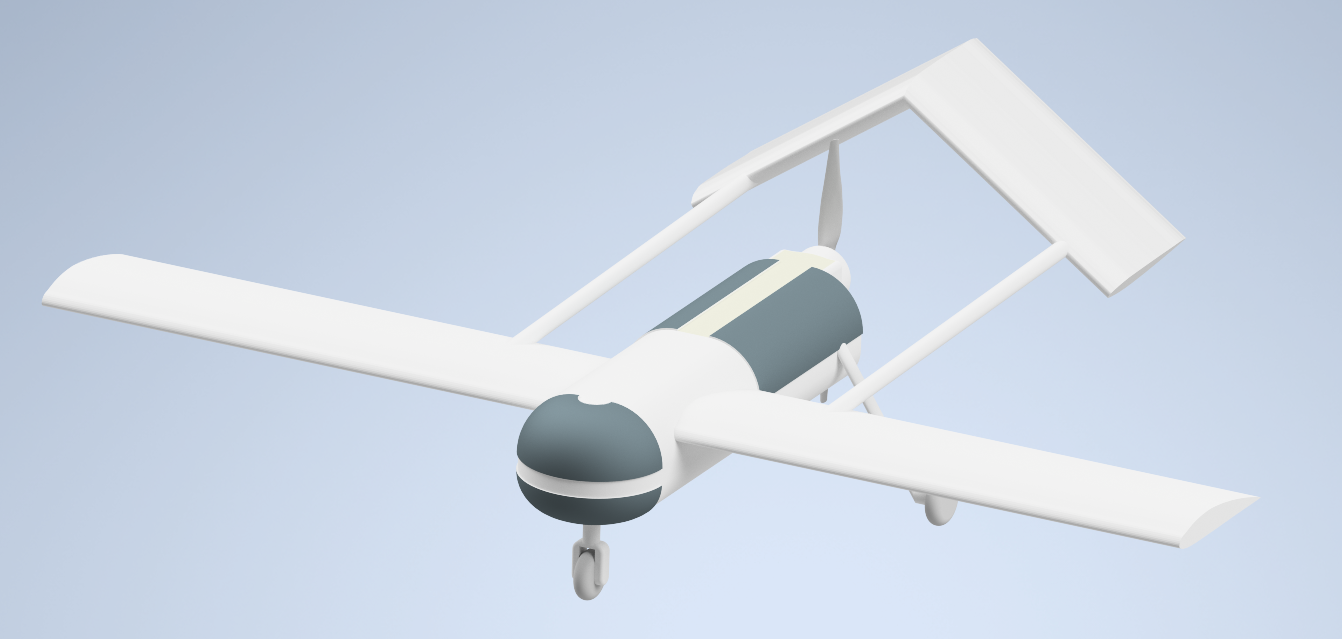
\includegraphics[width=6 in]{Media/Drone.png} % Placeholder for technical drawings
		\caption{Longitudinal cross-section of the LAHE UAV}
	\end{figure}
	
	\subsubsection{Front Cross-Section Layout}
	The fuselage is comprised mostly of a continuous cross-section. The top half of the cross-section is reserved for payload. The bottom half has a sizable battery bay, a wiring bay, and a reserve bay. The battery is placed to lower the center of gravity as much as possible and thereby maximizing stability with a high wing design. The wiring bay is reserved for necessary power and avionics buses that run through the aircraft. Again maximizing mission flexibility, the reserve bay is left empty. The reserve bay can be augmented to place additional payload or batteries. 
	\begin{figure}[h!]
		\centering
		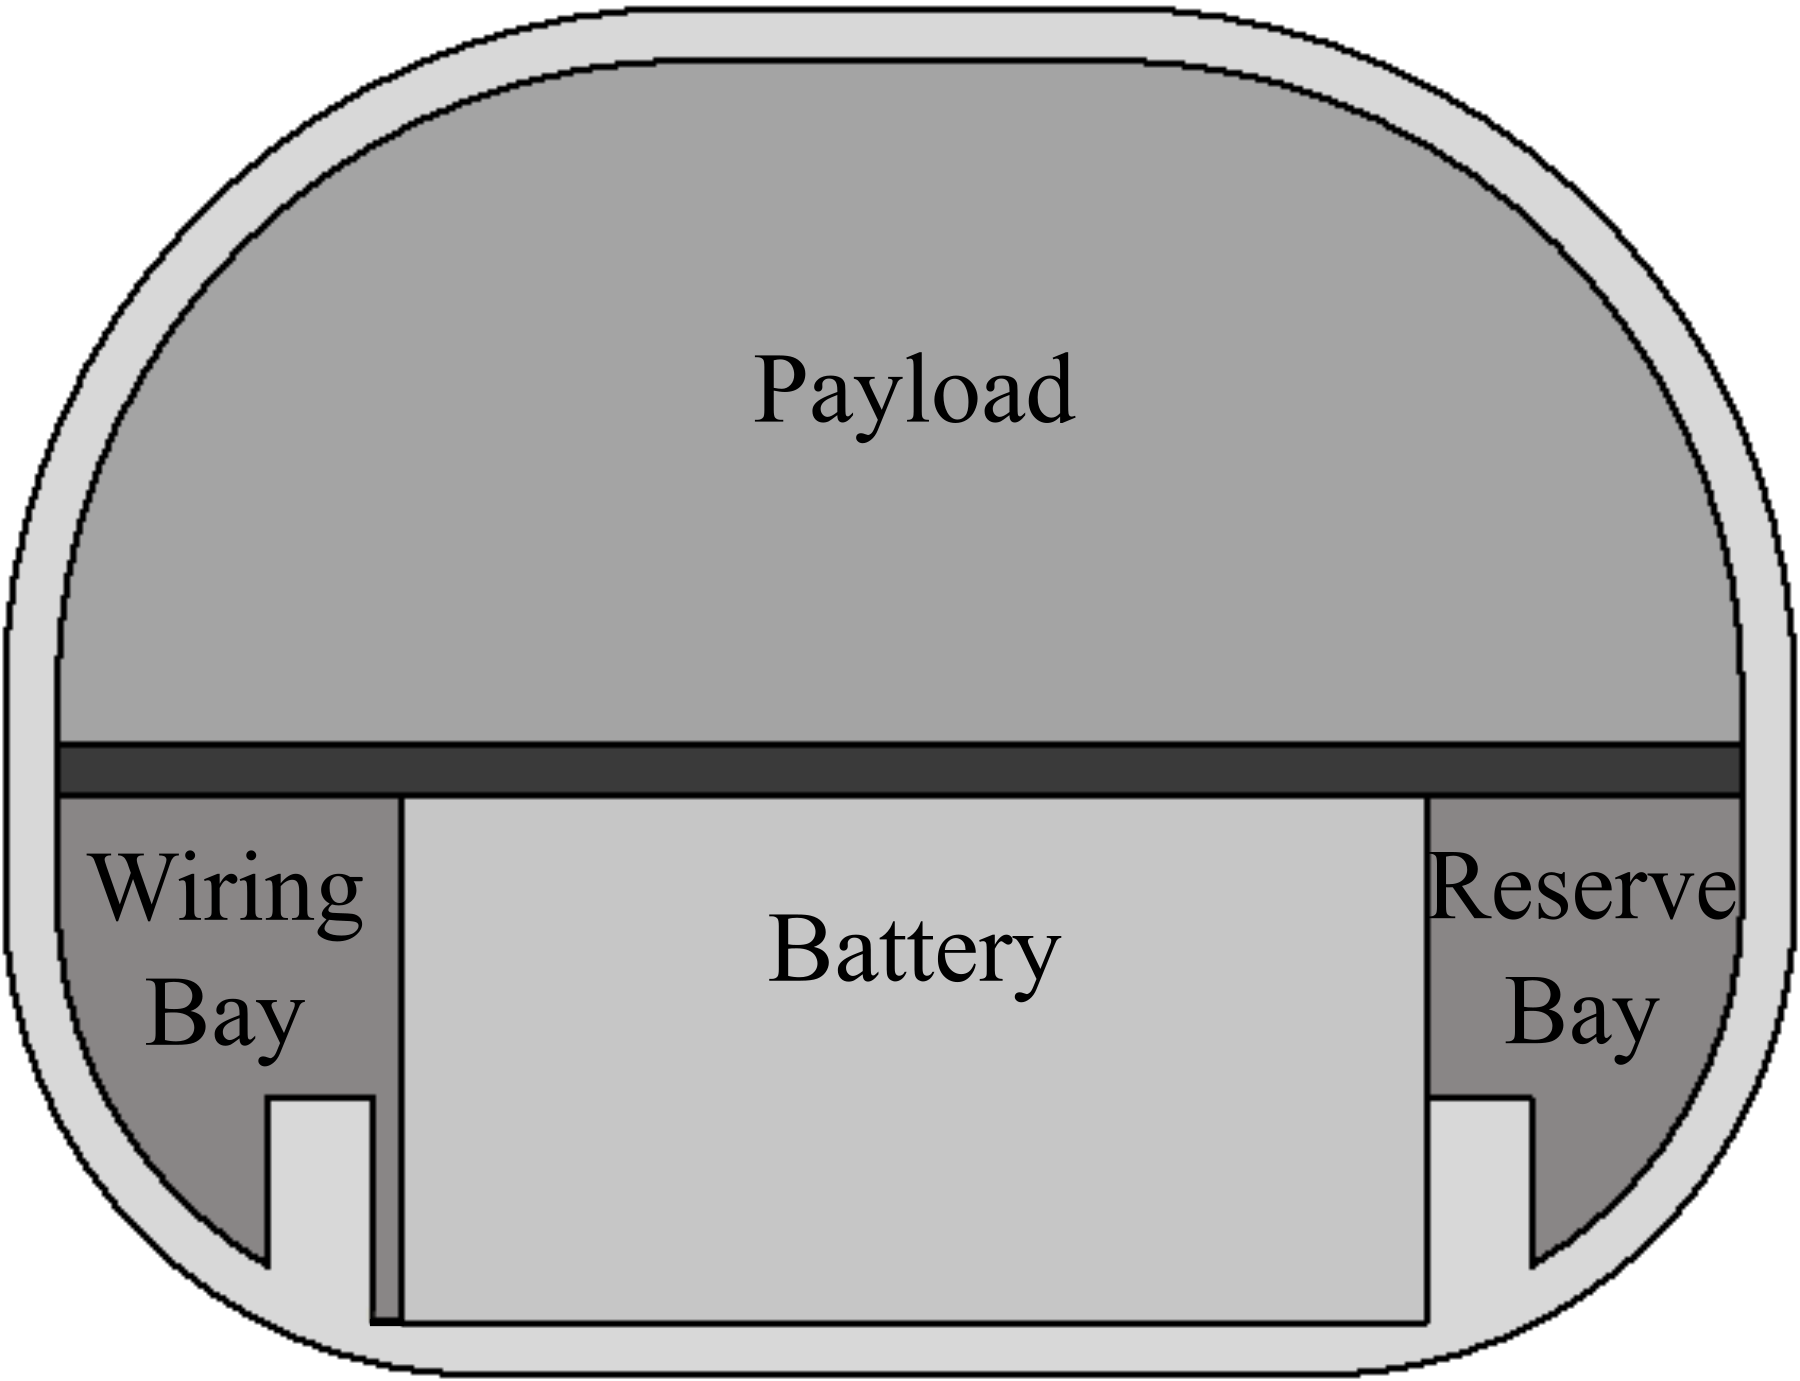
\includegraphics[width=6 in]{Media/FrontCrossSection.png} % Placeholder for technical drawings
		\caption{Longitudinal cross-section of the LAHE UAV}
		\label{figure6}
	\end{figure}
	
	Note on figure \ref{figure6} the gap between the two posts and the battery; this gap was implemented to leave room for thermal swelling, which is a common phenomenon of lithium polymer batteries. Lithium batteries, depending on their exact makeup, can expand by as much as 5\%\cite{}. 
	
	%compare payload size of similar drones here
	
	\subsubsection{Side Cross-Section Layout}
	The side cross-section was primarily sized to accommodate 2-40 Ah Batteries in addition to an avionics bay. Preliminary literature review suggests that for similar design requirements approximately 80 Ah is needed.
	
	\begin{table}[h]
		\centering
		\caption{Aircraft Specifications}
		\begin{tabular}{|l|l|l|l|}
			\hline
			\textbf{Aircraft} & \textbf{Battery Capacity} & \textbf{Payload} & \textbf{Endurance} \\ 
			\hline
			SITARIA E & 73.5 Ah & 8.82 lb & 3 h \\ 
			\hline
			\textbf{LAHE UAV} & \textbf{80 Ah} & \textbf{11.02 lb} & \textbf{3 h} \\ 
			\hline
			BOREY 20 & 83 Ah & 11.02 lb & 5 h \\ 
			\hline
		\end{tabular}
	\end{table}
	
	The fuselage was designed with ease of access in mind. The entire top will be removable to allow access to the payload bay. By removing the central plate, it is possible to also access the battery bays and the avionics. The motor is readily removable from the rear for maintenance.
	
	\begin{figure}[h!]
		\centering
		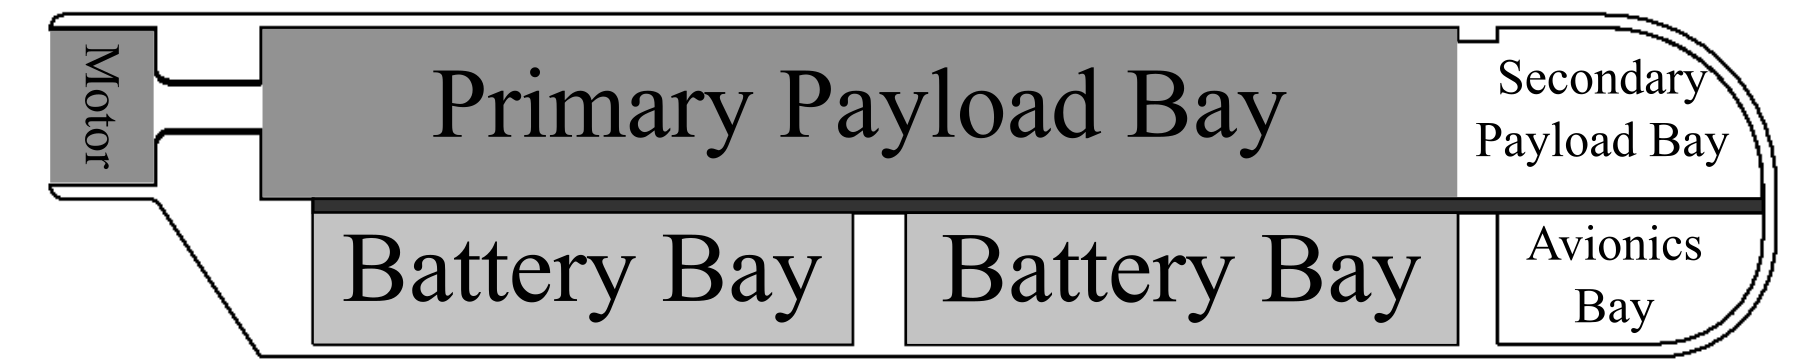
\includegraphics[width=6 in]{Media/SideCrossSection.png} % Placeholder for technical drawings
		\caption{Latitudinal cross-section of the LAHE UAV}
	\end{figure}
	
	\subsubsection{Design Flexibility}
	The LAHE UAV is designed with flexibility in mind. In exchange for removing a battery, it is possible to convert a battery bay into additional payload space. The ability to rapidly swap batteries allows operators to quickly tailor the LAHE UAV to an entire suite of mission types. Each 40Ah battery weighs 8.82 lb; by removing one and adding 8.82 lb of payload, the endurance approximately halves but the payload nearly doubles. It is also possible to replace the 40Ah batteries with smaller capacity batteries to get more fine control of the payload vs range curve. 
	
	Below are a few example configurations along with outlines of mission use cases.
	
	\begin{figure}[h!]
		\centering
		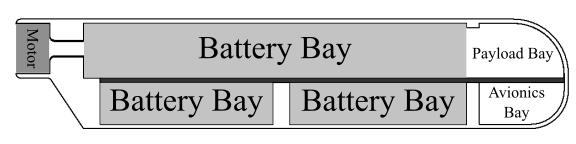
\includegraphics[width=6 in]{Media/UltraEnduranceConfig.png} % Placeholder for technical drawings
		\caption{Longitudinal cross-section of the LAHE UAV}
	\end{figure}
	
	If the weight of the sensor package is minimal but range or endurance is critical, the primary payload bay can be exchanged in lieu of more batteries. This would leave the secondary payload bay as the only payload bay. This configuration could potentially double or triple endurance.
	
	\newpage
	
	\begin{figure}[h!]
		\centering
		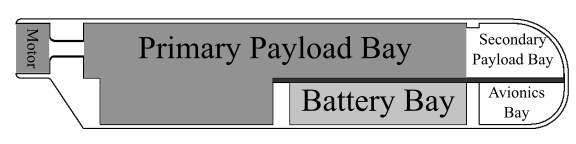
\includegraphics[width=6 in]{Media/HighPayloadConfig.png} % Placeholder for technical drawings
		\caption{Longitudinal cross-section of the LAHE UAV}
	\end{figure}
	
	For volumetrically large payloads on missions where endurance is less of a concern, a battery can be removed along with its panel to increase the primary payload bay by 50\%.
	
	\begin{figure}[h!]
		\centering
		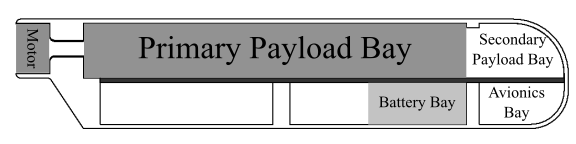
\includegraphics[width=6 in]{Media/HighDensityPayloadConfig.png} % Placeholder for technical drawings
		\caption{Longitudinal cross-section of the LAHE UAV}
	\end{figure}
	
	For missions with dense payloads where endurance is of no concern, the two 40 Ah batteries can be replaced with one 20 Ah battery. This would reduce the flight time to as little as 20 minutes but would allow for very heavy payloads.
	
	\subsubsection{Landing Gear}
	A fixed tricycle landing gear configuration with a slight nose-up cant was elected for this aircraft. Moving 32.81 to 98.43 ft/s, aerodynamic drag contributes significantly less than structural weight to the aircraft's overall endurance; fixed landing gear with no nacelle minimizes weight compared to moving gear or gear with nacelles. A 2° nose-up cant will increase the lift coefficient of most wings, thereby decreasing take-off runs. On landing, the nose-up cant reduces the risk of nose-over flipping, which could pose catastrophic damage to sensitive equipment in the nose. To provide clearance to the propeller with an approximately 1.38 in margin, a nominal landing gear height of 5.12 in was chosen. Technical drawings attached to the report outline in detail the exact clearances of the landing gear system. 
	
	\newpage
	
	\appendix

	
	
	\begin{figure}[h!]
		\centering
		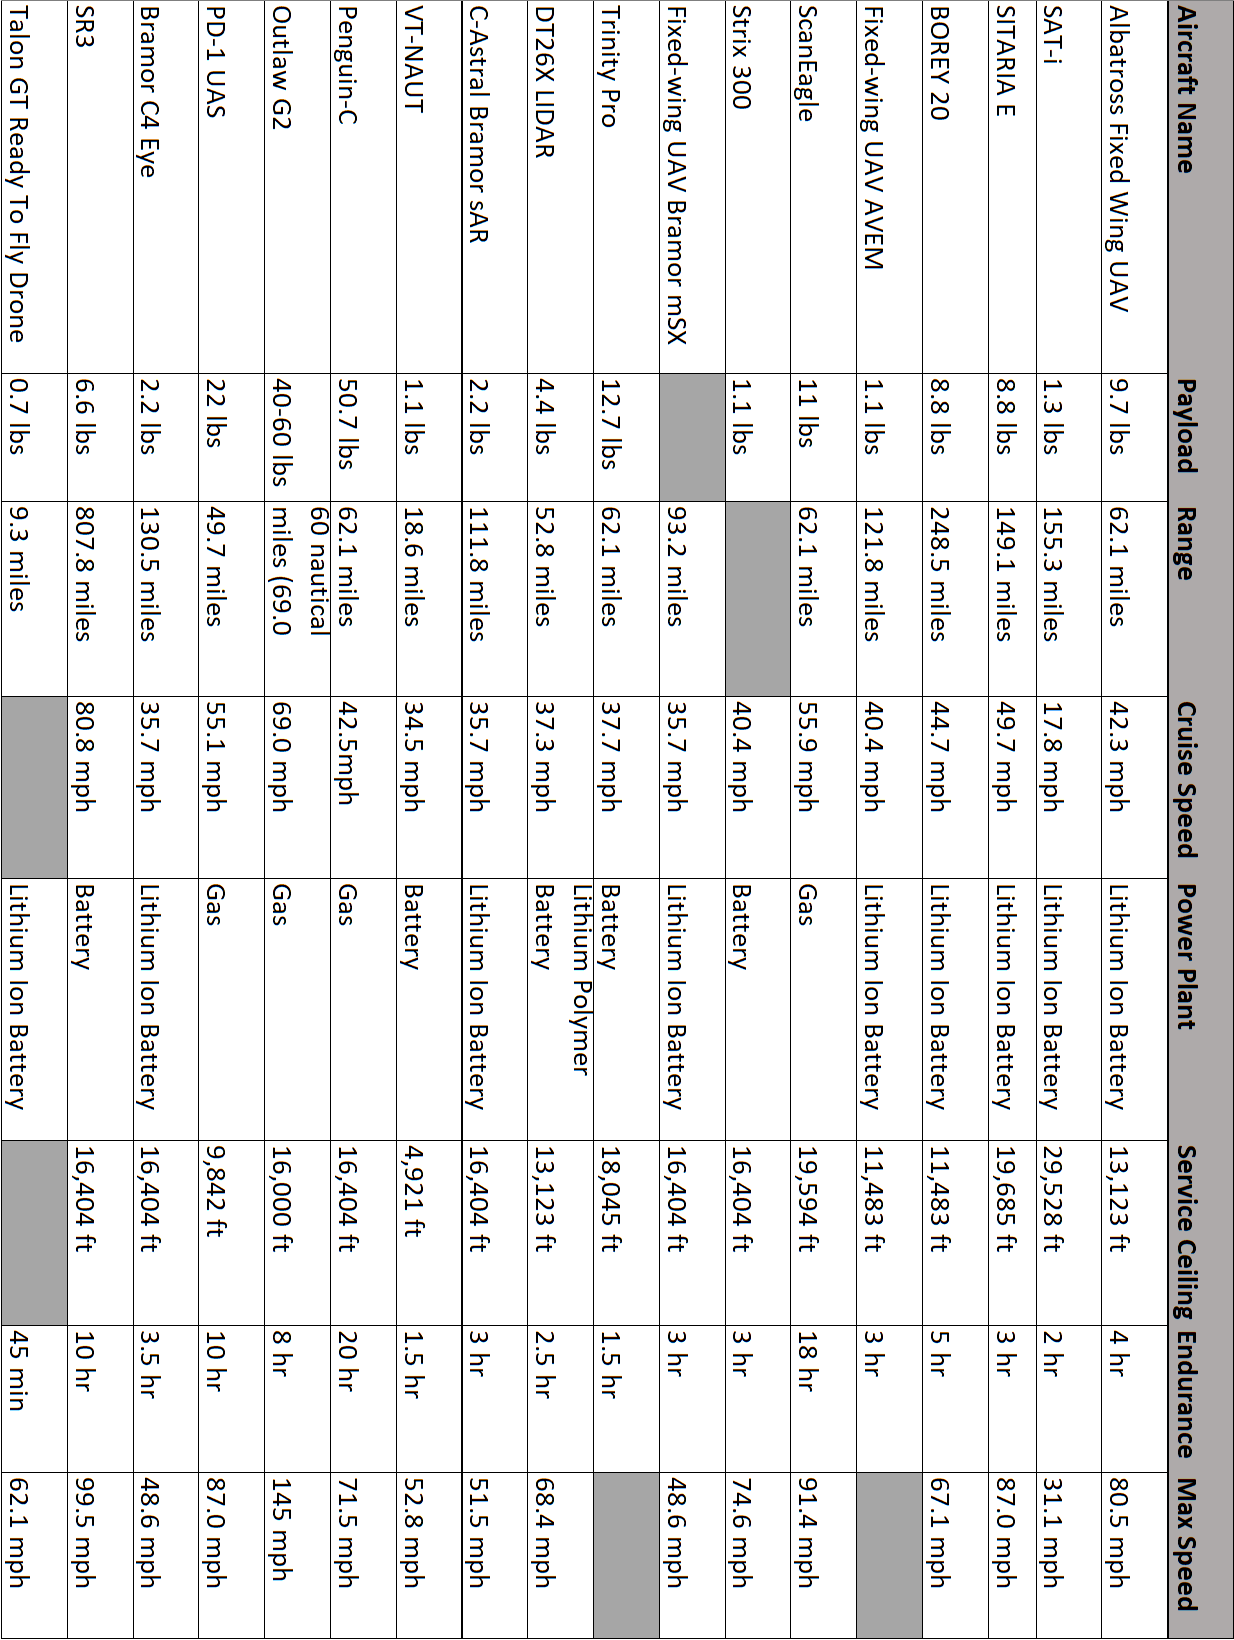
\includegraphics{Media/Table.png} % Placeholder for technical drawings
		\caption{Longitudinal cross-section of the LAHE UAV}
	\end{figure}


	
	\newpage
	
	\begin{thebibliography}{9}
		\bibitem{faa_2023}
		FAA, "14 CFR Part 48," \url{https://www.faa.gov/air_traffic/publications/atpubs/aim_html/chap11_section_2.html}, 2023.
	\end{thebibliography}
	
\end{document}
